\section{Methodology}
\label{sec:methodology}

% Avsnitt om hva slags type review dette er og hvorfor vi har valgt den typen
To ensure reproducible and unbiased results, this review follows a structured methodology. As noted by \textcite{tranfield_et_al}, traditional literature reviews often lack systematic rigor, making it challenging to determine the validity of their conclusions. To address this issue, each stage of the review was conducted systematically, guided by established literature review frameworks, particularly \textcite{snyder_2019} and \textcite{marzi_et_al_2024}. Given that the purpose of the review is to map the current use and impact of probabilistic AI models for uncertainty estimations in financial time series the chosen style is what \textcite{snyder_2019} calls a structured, systematic literature review (SLR) to ensure that the review is both exhaustive and focused on capturing the rapid development in the field and addressing the identified research gaps. The exact process is outlined below.


% Avsnitt om databasevalg
\textbf{Database Selection} \\
When doing a systematic review, it is important to conduct search in a sufficient number of databases to ensure that all relevant articles are retrieved \parencite{hiebl_2021}. Furthermore, it is critical that the databases are relevant for the researched topic \parencite{marzi_et_al_2024}. In order to comprehensively capture all potentially relevant literature, this review utilized multiple well-establish databases: SCOPUS, Web of Science, IEEE Xplore and ProQuest. SCOPUS and Web of Science were chosen due to their extensive coverage and comprehensive indexing of academic literature within a wide range of fields, as well as being the most extensively used databases for reviews \parencite{marzi_et_al_2024}. IEEE Xplore was included being a leading database for review articles in the fields of computer science and engineering \parencite{suhaimi2020systematic, carvalho2019systematic, cavacini2015best}, while ProQuest is another large academic database utilized in line with \textcite{gunnarsson2024}. All chosen databases allowed for advanced search queries without limitations on the number of clauses, in contrast to for example Google Scholar and ScienceDirect. 

% Avsnitt om søkekriterier
\textbf{Search Strategy and Criteria} \\
A comprehensive search and filtering strategy was developed to ensure the review covered all relevant literature. The search criteria were designed to ensure that as many articles relevant to the research questions as possible were included, as a narrow search query in this phase can lead to involuntary exclusion of relevant documents \parencite{marzi_et_al_2024,kuhrmann2017pragmatic, williams2021reexamining}. By requiring articles to match at least one term in four different clauses, the intention was to ensure that every article was (1) within the field of AI, (2) about probabilistic modeling, (3) about forecasting, and (4) within finance. Table \ref{table:keywords_used} shows all key words included within each clause. Conference papers, book chapters, editorials, and early access/unfinished papers were excluded to maintain a focus on peer-reviewed journal articles, as these can be regarded validated knowledge having undergone a peer-review process ensuring reliability \parencite{marzi_et_al_2024, hota2022hybrid}. Only English articles are included. The exact search queries are shown in Appendix \ref{appendix:search_queries}. 

\begin{table}[H]
    \centering
    \caption[Keywords used in database search queries]{Keywords used in database search queries across four key areas. Papers must match at least one term in each of the four categories to be included in the sample.}
    \label{table:keywords_used}
    \begin{adjustbox}{width=0.5\textwidth,center}
    \begin{tabular}{p{0.15\textwidth}p{0.35\textwidth}}
        \toprule
        \textbf{Category} & \textbf{Keywords} \\
        \midrule
        (1) Artificial Intelligence (AI) & \texttt{AI, ML, Artificial intelligence, Machine learning, Deep learning, Reinforcement learning, Supervised learning} \\
        \addlinespace
        (2) Probabilistic Modeling & \texttt{Probabilistic, Uncertainty quantification, Prediction interval*, Confidence interval*, Distributional forecast, Bayesian, Gaussian process, Undirected graphical model*, Markov Network*, Markov random field*, Probabilistic Graphical Model*, Variational inference, Monte Carlo inference, Hidden Markov model*, Gaussian mixture model*, Variational Autoencoder*, Dirichlet Process} \\
        \addlinespace
        \text{(3) Forecasting} & \texttt{Forecast*, Predict*, Estimat*} \\
        \addlinespace
        \text{(4) Finance} & \texttt{Cryptocurrency, Bitcoin, Foreign exchange, Forex, Equity market*, Stock price*, Stock market*, Commodities, Value-at-risk, Value at risk, CVaR, Expected shortfall, Financial time series, Stock trend*, Implied volatility, Realized volatility, (Volatility AND financ*)} \\
        \bottomrule
    \end{tabular}
    \end{adjustbox}
\end{table}

The search was conducted across all the databases in October 2024, yielding a combined initial search result of 485 articles from all databases. The search results were then merged, and duplicates were removed, resulting in 275 unique articles. 

\begin{figure}[H]
    \centering
    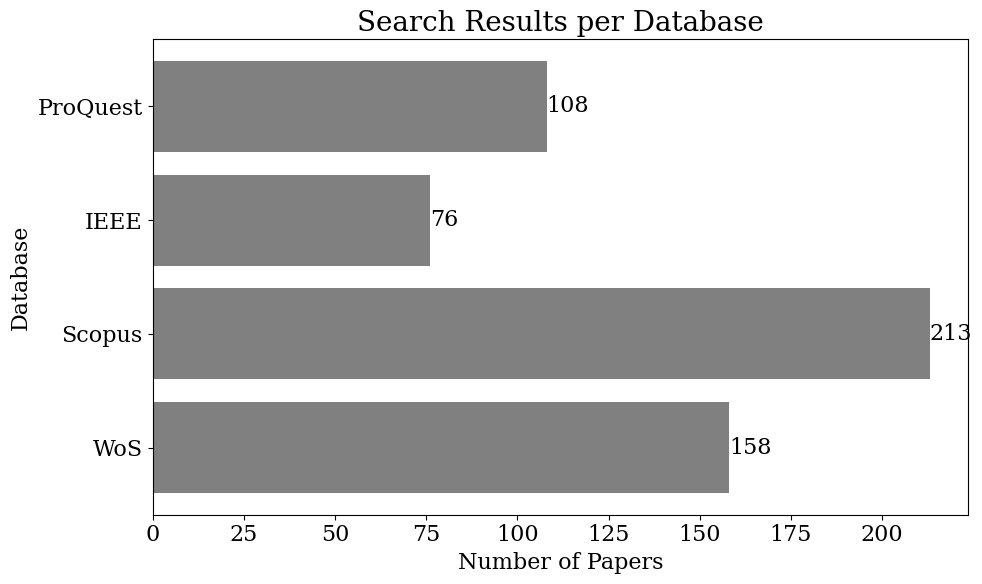
\includegraphics[width=1\linewidth]{Images/search_sample_by_database.png}
    \caption{Number of results in each database based on search queries}
    \label{fig:search_sample_by_database}
\end{figure}



% Avsnitt om screening
\textbf{Screening Process: Phase 1} \\
After obtaining the initial set of papers, phase 1 screening process started. In this stage, the purpose was to remove articles irrelevant to the research questions to be addressed in the review. This was done in a systematic manner, by defining three criteria for inclusion:

\begin{enumerate}
    \item The article must discuss a model that predicts the price of some financial instrument (e.g. a stock, an option, an index, etc.)

    \item The model is an AI or machine learning model, i.e. more complicated than traditional statistical or econometric models

    \item The model must be able to provide more than a point prediction, i.e. it includes either variance or a distribution or some other financial risk measure such as VaR
\end{enumerate}

[.. legge inn noe om hvordan vi har behandlet commodity-priser/futures ..]

[.. legge inn noe om hvordan vi har behandlet klassifiseringsmodeller ..]

To make the screening process more efficient, a large language model (``o1-mini'' from OpenAI) was given the title and abstract of each article and tasked with generating a short summary and assessing compliance with each criteria. Subsequently, the results from the language model, along with the title, abstract and a link to the full article was given to a human to make a decision on whether to include or exclude each article. Through this process, we were able to quickly make decisions on obvious cases, and do a more thorough assessment where we potentially read the full text in cases of doubt, thus enabling us to screen a large number of articles in a short amount of time, and making thorough assessments that were not based solely on the title and the abstract. The exact process is outlined in Appendix \ref{appendix:screening_process_with_ai}. Through this process, the number of articles in the sample was reduced from 275 to 113.

% Avsnitt om snowball effect - XX articles were added to sample by snowball effect
To ensure no key contributions to the field were overlooked, a snowball sampling technique where the references of included paper were checked for additional relevant papers, was applied as recommended by \textcite{marzi_et_al_2024}. This resulted in X additional articles added to the sample. 


% Avsnitt om den initielle analysen (taggingen)
\textbf{Data extraction and Analysis: Phase 2 } \\
Once the final dataset of articles was established, we evaluated each article thoroughly and extracted data on key information: the type of AI model used, target variable, type of uncertainty captured and metric used for assessing model performance, particular in terms of uncertainty estimates. 

Each article was tagged and categorized based on these variables which were summarized in a structured format for subsequent analysis and descriptive analysis. Upon further and more detailed evaluation of the sample articles, 49 articles was excluded based the exclusion and inclusion criteria presented earlier. 
Therefore, the final sample size of included articles presented in this paper is 64 articles. Figure \ref{fig:screening_and_cleaning_funnel} illustrates how the sample size was reduced down through the cleaning and screening. 

  \begin{figure}[H]
      \centering
      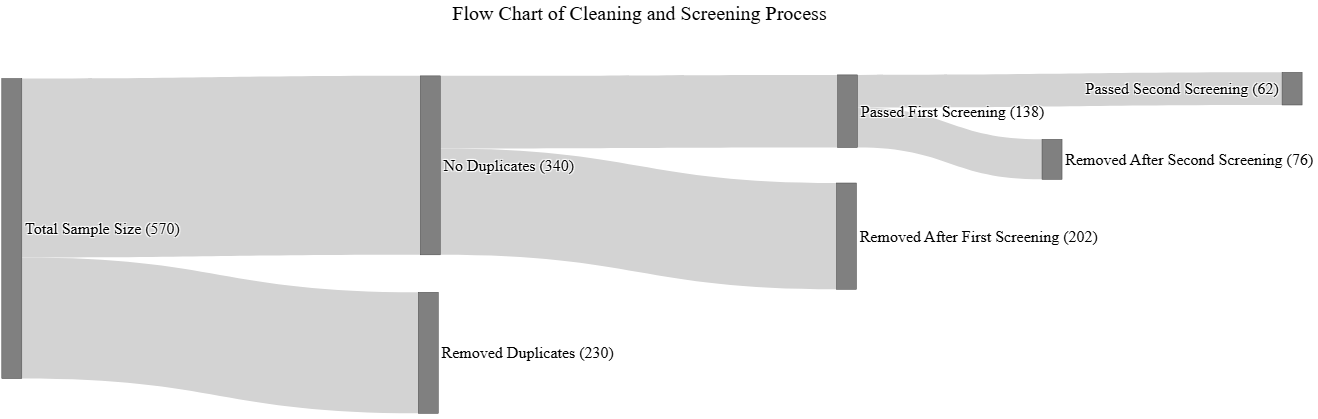
\includegraphics[width=1\linewidth]{Images/screening_funnel.png}
      \caption{Flow chart illustrating the sample size throughout cleaning and screening phases}
      \label{fig:screening_and_cleaning_funnel}
  \end{figure}


  % Avsnitt om hvordan deskriptiv statistikk ble laget og hvorfor, inkl. analysen som viste at de sjeldent referer til hverandre, med referanse til den B-SLR-artikkelen
\textbf{Descriptive Statistics and Analysis}\\
Descriptive statistics and analysis were generated using a Python Jupiter Notebook. Pandas was used for data manipulation and categorization, and Matplotlib for data visualizations and plotting. All code used for the analyses is disclosed and available for reproducibility at XX [link to GitHub repository]. 

% Avsnitt om den videre analysen (altså breakdown by model, by target variable, etc.): hvorfor og hvordan har vi gjort det?
\textbf{Approach for Further Analysis}\\
The further analysis of the articles follows a structured breakdown along several dimensions to analyze and review the literature on probabilistic AI and uncertainty estimation in financial time series. The analysis is broken down by descriptive statistics, model, target variable, asset and type of uncertainty. Each section will provide insights that address the research questions directly to provide a clear understanding of how current literature address the use of probabilistic AI to improve uncertainty estimation in financial time series. These are also dimensions commonly used in other reviews within the field, such as those by \textcite{Blasco_et_al_2024} and XX, to provide a structured framework to effectively analyse and evaluate the current state of the field. 

